\documentclass[10pt]{article}

\usepackage{graphicx}
\usepackage{hyperref}

\begin{document}

\title{COP290: Assignment-1 Documentation}
\author{Aviral Jain : 2013CS10215\\Rakshak Satsangi : 2013CS10250\\
}
\date{\today}
\maketitle

\hypersetup{
    colorlinks=true,
    linkcolor=blue,
    filecolor=magenta,      
    urlcolor=cyan,
}
\tableofcontents

\newpage 
\section{External Design}
	The application will feature a screen where n balls (n specified by the user) will move colliding elastically with the boundaries and other balls. The balls will start from random positions on the screen with random speeds in the beginning. The user will be able to change the ball speed of any ball from a pause screen obtained from a key click. After that, the balls will start moving again from random positions with updated speeds. Speed will be on a scale of 1 to 5. The ball sizes will be fixed and can only be changed from the source code. Based on the ball sizes, we will find a maximum number of balls possible, and the user shall not specify n to be above this number.
\begin{center}
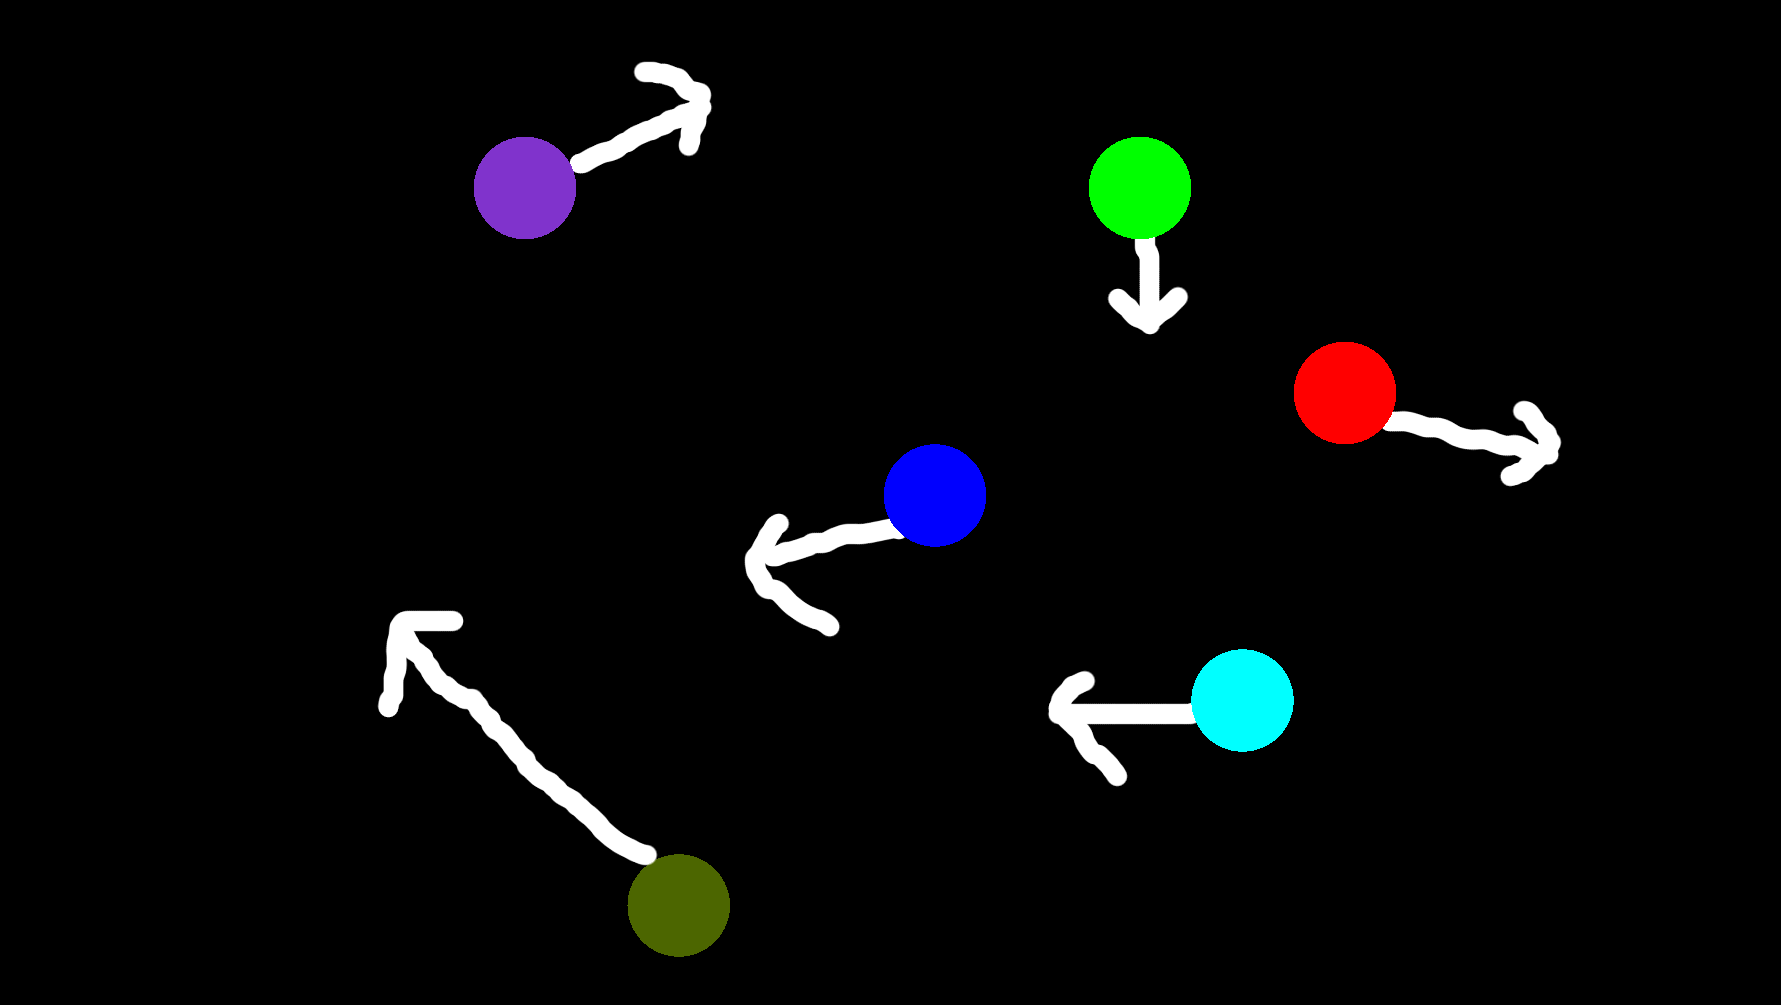
\includegraphics[width = 5in]{screen.png}\\
\textsf{Image displaying n=6 balls at random positions on screen with variable speeds in random directions}
\end{center}

\section{Sub Components in Design}
	\subsection{GUI}
		GUI will be implemented using openGL. 
		\subsubsection{Displaying N balls}
			Circle is not a primitive/built-in shape in openGL. We define our own function \texttt{DrawCircle} to draw a circle which draws a polygon with large number of sides taking co-ordinates of centre as argument.
		\subsubsection{Motion of balls}
			The  \texttt{Display} function will be called at a particular frequency (say every 30 milliseconds). In each call, it upadates the position of ball(co-ordinates of center) as per the rules of Physics as discussed in Section 2.2. The ball is then drawn at the new position. 
		\subsubsection{User Controlled speeds of each ball}
			
			On MouseClick anywhere inside the window, the balls would come to standstill i.e., the screensaver would get paused. The background colour would be adjusted to show nice effects.
			
			Then we can select any ball by clicking on the ball and use arrow keys to increase/decrease x/y-speeds. On selection the colour of ball would be adjusted to show nice effects. The screensaver would resume on pressing the keys, thus the effect of pressing the keys would be seen simultaneously. There would be a lower and upper limit on the speeds. 
			
			To deselect the ball, user would need to click on empty area on the window.
		\subsubsection{Special Effects}
			On collision of a ball with another ball, we could produce a temporary star emerging in between them and lasting for few moments.
	\subsection{Physics Governing the Motion of Balls}
		The balls would follow the Laws of Elastic Collision. We would assume all balls to be of same masses.
		\subsubsection{Collision with Wall}
			In case of collision with wall, the direction of balls would get reversed along the line of impact (x-axis for side walls and y-axis for top \& bottom walls). 
			The speed of ball in tangential direction (perpendicular to the line of impact) would be unchanged.
			
			\begin{center}
			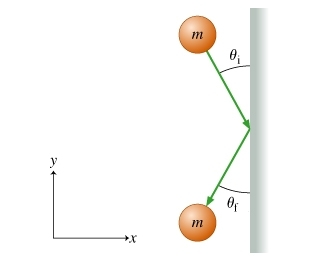
\includegraphics[width = 1.5in]{cwall.jpg}\\
			\textsf{Ball colliding elastically with a wall}
			\end{center}
			

		\subsubsection{Collision among balls}		
			Along the direction of impact (which is the line joining the centres of two balls) the velocities would get interchanged.
			The velocities along the tangential direction would be unchanged.
			\begin{center}
			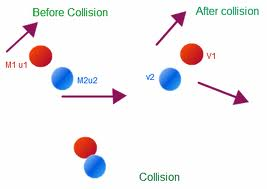
\includegraphics[width = 1.5in]{cball.jpeg}\\
			\textsf{Ball colliding elastically with another ball}
			\end{center}
	\subsection{Inter Thread Synchronisation}
	Why to use pthreads?
	The motivation behind using multiple threads is to do parallel processing instead of single-threaded program. It would perform the calculations of each ball simultaneously (parallel computation) and avoid any lags in preview of screensaver.
	
	Pthreads are used to store data for every ball. Thread synchronization using mutex will be required for effecting collisions. One-to-one communication model will be used.\\\\
	\textsc{Calculations:}
	\begin{enumerate}
	\item
	We would check for the co-ordinate of extreme right, left, top, bottom of ball to be within the range of viewport. If not, then it means that the ball collides with the wall and the velocity of ball must be updated in accordance with laws of elastic collision.
	\item
	We would check whether the distance between the centers of two balls exceeds the sum of their radii. If not, it means that the balls have collided and we would update the velocities of the balls in accordance with the laws of elastic collision. 	
	\end{enumerate}

\section{Test Cases}
	\subsection{Testing of GUI}
		We woulld change the window size by dragging the edges and check for two things.
		\begin{itemize}
		\item Distortion of shape of ball
		\item Relative position of ball must remain same w.r.t walls.
		\end{itemize}
		We have used \texttt{gluOrtho2D} function to adjust the aspect ratio of clipping area in accordance with the window.
	\subsection{Testing of Motion of balls}
		\begin{itemize}
		\item First, we would take a single ball and check its collision with wall. The ball should follow the laws of elastic collision. It must not go outside the window area.
		\item Next, we would take multiple balls and check for collision of balls among themselves. The balls must follow the laws of elastic collision. They should not overlap or pass through each other. No ball must escape the window.
		\item Some boundary condition must be taken care of to provide a realistic view, for example, there must not be any delay/pause after a collision.
		\item We would slow down the frequency of the call of \texttt{Display} function to analyse frame by frame.
		\end{itemize}
\section{Interaction of Sub Components}
	A function for implementing physics would update the position of center of ball at every step in accordance to the laws of motion, especially laws of elastic collision.
	
	A function for implementing GUI would draw the balls taking information of co-ordinates of center from the previously defined function for implementing physics.
	
	The thread corresponding to each ball would parallely process these two functions.


\end{document}